\documentclass{standalone}

% put this in your preamble
\usepackage{tikz}
\usepackage{amssymb}

\begin{document}

% put this tikzpicture block in your LaTeX document where you want the figure
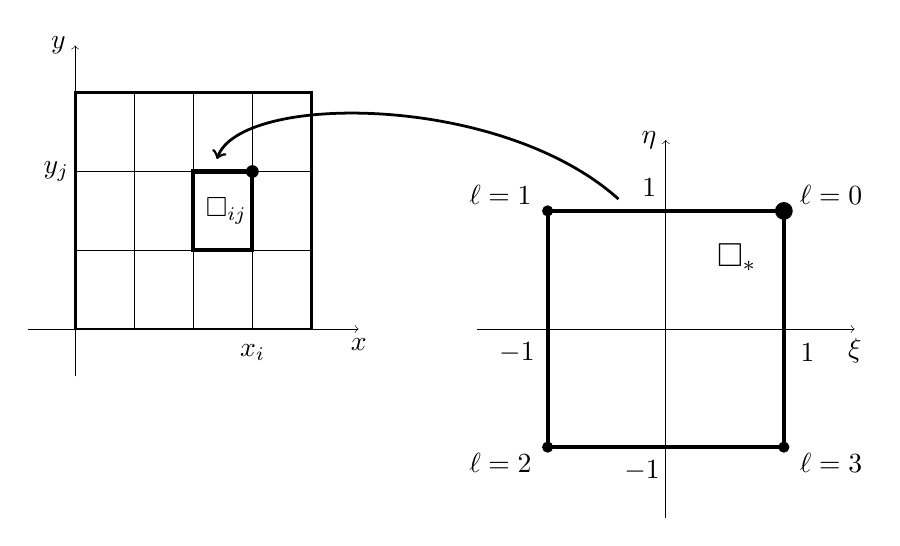
\begin{tikzpicture}[scale=3.0]
% (x,y) elements
  \draw[->,very thin] (-0.2,0.0) -- (1.2,0.0) node[below] {$x$};
  \draw[->,very thin] (0.0,-0.2) -- (0.0,1.2) node[left] {$y$};
  \draw[line width=1.0pt] (0.0,0.0) -- (0.0,1.0) -- (1.0,1.0) -- (1.0,0.0) -- cycle;
  \pgfmathsetmacro\fourth{1.0/4.0}
  \pgfmathsetmacro\third{1.0/3.0}
  \pgfmathsetmacro\twothird{2.0/3.0}
  \draw[xstep=\fourth,ystep=\third,black,thin] (0.0,0.0) grid (1.0,1.0);
  % outline an element
  \draw[line width=1.5pt] (0.5,\third) -- (0.75,\third) -- (0.75,\twothird) -- (0.5,\twothird) -- cycle;
  \node at (0.64,0.5) {$\square_{ij}$};
  \node at (0.751,-0.1) {$x_i$};
  \node at (-0.08,\twothird) {$y_j$};
  \filldraw (0.75,\twothird) circle (0.7pt);

% (xi,eta) reference element
% origin of axes at (2.5,0.0) and square has half-width 0.5
  \draw[->,very thin] (1.7,0.0) -- (3.3,0.0) node[below] {$\xi$};
  \draw[->,very thin] (2.5,-0.8) -- (2.5,0.8) node[left] {$\eta$};
  \draw[line width=1.5pt] (2.0,-0.5) -- (3.0,-0.5) -- (3.0,0.5) -- (2.0,0.5) -- cycle;
  \node at (3.1,-0.1) {$1$};
  \node at (1.87,-0.1) {$-1$};
  \node at (2.43,0.6) {$1$};
  \node at (2.4,-0.6) {$-1$};
  \node at (2.8,0.3) {\large $\square_\ast$};
  \filldraw (3.0,0.5) circle (1.0pt) node[xshift=6mm,yshift=2mm] {$\ell=0$};
  \filldraw (2.0,0.5) circle (0.6pt) node[xshift=-6mm,yshift=2mm] {$\ell=1$};
  \filldraw (2.0,-0.5) circle (0.6pt) node[xshift=-6mm,yshift=-2mm] {$\ell=2$};
  \filldraw (3.0,-0.5) circle (0.6pt) node[xshift=6mm,yshift=-2mm] {$\ell=3$};
% arc:
  \draw[->,line width=1.0pt] (2.3,0.55) .. controls (1.8,1.0) and (0.7,1.0) .. (0.6,0.72);
\end{tikzpicture}
\end{document}
